\documentclass{beamer}
%
% Choose how your presentation looks.
%
% For more themes, color themes and font themes, see:
% http://deic.uab.es/~iblanes/beamer_gallery/index_by_theme.html
%
\usetheme[style=simple,nat]{Frederiksberg}
\usefonttheme{serif}  

\usepackage{Nikolai}
\usepackage[english]{babel}
\usepackage[super]{nth}


\title[Bachelors Thesis]{Visualization of Concepts in Condensed Matter Physics}
\author{Nikolai Plambech Nielsen}
\institute{Niels Bohr Institute}
\date{\nth{27} of June, 2018}

\begin{document}

\begin{frame}
  \titlepage
\end{frame}


\section{Outline}
\begin{frame}{Outline}
\begin{itemize}
  \item Introduction
  \item Background
  \item Lattices and crystal structure
  \item The reciprocal lattice and scattering
  \item Band structure
\end{itemize}
\end{frame}



\section{Introduction}
\begin{frame}{Introduction}
\end{frame}


\section{Background}
\begin{frame}{Background}
Bloch's theorem
\begin{equation}
	\psi(\V{r}) = e^{i \V{k}\D \V{r}} u(\V{r})
\end{equation}
\end{frame}


\section{Lattices and crystal structure}
\begin{frame}{Lattices and crystal structure}
\begin{equation}
	\V{R} = \sum_{i = 1}^{d} n_i \V{a}_i
\end{equation}
\begin{figure}[H]
	\centering
	\begin{minipage}{.4\textwidth}
		\centering
		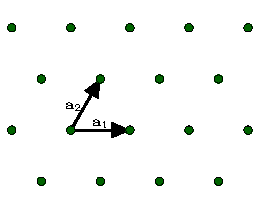
\includegraphics[width=\linewidth]{figures/triangular.pdf}
		\captionof{figure}{A triangular lattice. $ \V{a}_1 = a\D(1,0)$, \\$\V{a}_2 = a\D(1/2, \sqrt{3}/2) $}
		\label{fig:triangular_lattice}
	\end{minipage}%
	\hfill
	\begin{minipage}{.4\textwidth}
		\centering
		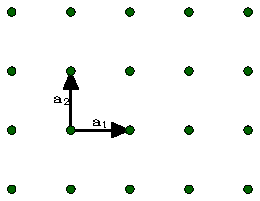
\includegraphics[width=\linewidth]{figures/square.pdf}
		\captionof{figure}{A square lattice. $ \V{a}_1 = a\D(1,0), \V{a}_2 = a\D(0,1) $}
		\label{fig:square_lattice}
	\end{minipage}
\end{figure}
\end{frame}


\begin{frame}{Lattices and crystal structure}
\begin{equation}
\V{R} = \sum_{i = 1}^{d} n_i \V{a}_i
\end{equation}
\begin{figure}[H]
	\centering
	\begin{minipage}{.4\textwidth}
		\centering
		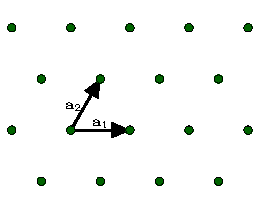
\includegraphics[width=\linewidth]{figures/triangular.pdf}
		\captionof{figure}{A triangular lattice. $ \V{a}_1 = a\D(1,0)$, \\$\V{a}_2 = a\D(1/2, \sqrt{3}/2) $}
		\label{fig:test1}
	\end{minipage}%
	\hfill
	\begin{minipage}{.4\textwidth}
		\centering
		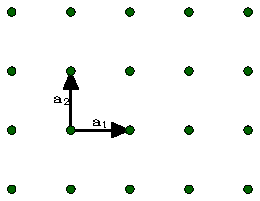
\includegraphics[width=\linewidth]{figures/square.pdf}
		\captionof{figure}{A square lattice. $ \V{a}_1 = a\D(1,0), \V{a}_2 = a\D(0,1) $}
		\label{fig:test2}
	\end{minipage}
\end{figure}
\end{frame}

\end{document}
